\documentclass[a4paper]{article}
\usepackage[fontsize=13pt]{scrextend}
\usepackage[utf8]{vietnam}
\usepackage{amsmath}
\usepackage{amsfonts}
\usepackage{xcolor}
\usepackage{titlesec}
\usepackage{mdframed}
\usepackage{amssymb}
\usepackage{pgf,tikz,pgfplots}
\usepackage{graphicx}
\graphicspath{ {figures/} }
\usepackage{array}
\usepackage{cases}
\usepackage{listings}
\usepackage{tabulary}
\usepackage{color}
\usepackage{float} 
\usepackage{hyperref}
\usepackage{multirow}
\usepackage{minitoc}
\pgfplotsset{compat=1.5}
\usepackage{mathrsfs}
\usetikzlibrary{arrows, calc}
\usepackage{fancyhdr}
\pagestyle{fancy}
\pagestyle{empty}
\definecolor{dkgreen}{rgb}{0,0.6,0}
\definecolor{gray}{rgb}{0.5,0.5,0.5}
\definecolor{mauve}{rgb}{0.58,0,0.82}
\lstset{frame=tb,
  language=C++,
  aboveskip=3mm,
  belowskip=3mm,
  showstringspaces=false,
  columns=flexible,
  basicstyle={\small\ttfamily},
  numbers=none,
  numberstyle=\tiny\color{gray},
  keywordstyle=\color{blue},
  commentstyle=\color{dkgreen},
  stringstyle=\color{mauve},
  breaklines=true,
  breakatwhitespace=true,
  tabsize=3
}
\renewcommand{\listfigurename}{Danh sách hình}
\renewcommand{\listtablename}{Tables}
\newcommand{\tabitem}{~~\llap{\textbullet}~~}
\usepackage[left=2cm,right=2cm,top=2cm,bottom=2cm]{geometry}
\author{Nguyễn Văn Lộc}
\newmdenv[linecolor=black,skipabove=\topsep,skipbelow=\topsep,
leftmargin=-5pt,rightmargin=-5pt,
innerleftmargin=5pt,innerrightmargin=5pt]{mybox}
\hypersetup{
    colorlinks=true,
    linkcolor=blue,
    filecolor=magenta,      
    urlcolor=red,
    pdftitle={Report},   
}
\begin{document}
\begin{titlepage}
\begin{mybox}
\begin{center}
\fontsize{12}{12}\selectfont
\textbf{ĐẠI HỌC QUỐC GIA THÀNH PHỐ HỒ CHÍ MINH}\\
\textbf{TRƯỜNG ĐẠI HỌC KHOA HỌC TỰ NHIÊN}\\
\textbf{KHOA CÔNG NGHỆ THÔNG TIN}
\end{center}
\vskip 1 cm
\begin{figure}[H]
\begin{center}

\includegraphics[scale=0.25]{images/logo}
\end{center}
\end{figure}
\vskip 1 cm
\begin{center}
\fontsize{18}{14}\selectfont
\textbf{ĐỒ ÁN MÔN HỌC}\\
\fontsize{26}{16}\selectfont
\textbf{TOÁN ỨNG DỤNG VÀ THỐNG KÊ}\\
\fontsize{18}{12}\selectfont
\textbf{ĐỀ TÀI: Bài toán khí hậu}\\
\textbf{Bài toán 1}
\end{center}
\vskip 1 cm
\fontsize{14}{12}\selectfont
\textbf{Giảng viên lý thuyết:} PGS.TS Nguyễn Đình Thúc\\
\textbf{Lớp:} 20TN\\
\textbf{Thành viên thực hiện:}
\begin{itemize}
\item 20120131 $-$ Nguyễn Văn Lộc
\item 20120536 $-$ Võ Trọng Nghĩa
\item 20120572 $-$ Nguyễn Kiều Minh Tâm
\end{itemize}
\vskip 3 cm
\begin{center}
\textbf{THÀNH PHỐ HỒ CHÍ MINH, THÁNG 3 NĂM 2022}
\end{center}
\end{mybox}
\end{titlepage}

\tableofcontents
\listoffigures
\listoftables
\newpage

\section*{Lời nói đầu}

\newpage

\section{Đặt vấn đề}
\subsection{Xác định và hình thức hóa mục tiêu của bài toán}
\textbf{Bài toán:} Phân tích dữ liệu về lượng mưa trung bình năm từ năm 1886 đến năm 2021 ở trạm Concordia Muni AP, Kansas, miền Tây Hoa Kỳ.\\
\textbf{Hình thức hóa mục tiêu của bài toán:} vẽ biểu đồ histogram, xác định các giá trị thống kê mẫu của dữ liệu rồi đưa ra nhận xét.

\subsection{Dạng bài toán}
Bài toán này thuộc dạng bài toán \textbf{Mô tả} (nêu ra các đặc trưng của dữ liệu).

\subsection{Đối tượng được chọn cho bài toán}
Dữ liệu về lượng mưa trung bình năm của trạm Concordia Muni AP.\\
Cột PRCP (cột BU) của tập tin \textbf{USW00013984.csv} trong thư mục \textbf{gsoy-latest}, lấy từ \href{https://www.ncei.noaa.gov/data/gsoy/archive/}{dataset về Global Summary of the Year của NOAA}.

\subsection{Phạm vi, mức độ, quy mô của bài toán}
Theo không gian: dữ liệu được xử lý trong bài toán đại diện cho bang Kansas của Hoa Kỳ.\\
Theo thời gian: dữ liệu được thu thập trong vòng 136 năm, từ năm 1886 đến năm 2021.

\section{Thu thập và xử lý dữ liệu}

\section{Phân tích, đánh giá và kết luận}
\subsection{Kết quả xử lý}
Dưới đây là hai biểu đồ thể hiện tập dữ liệu trên; bểu đồ đường và biểu đồ phân tán.
\begin{center}
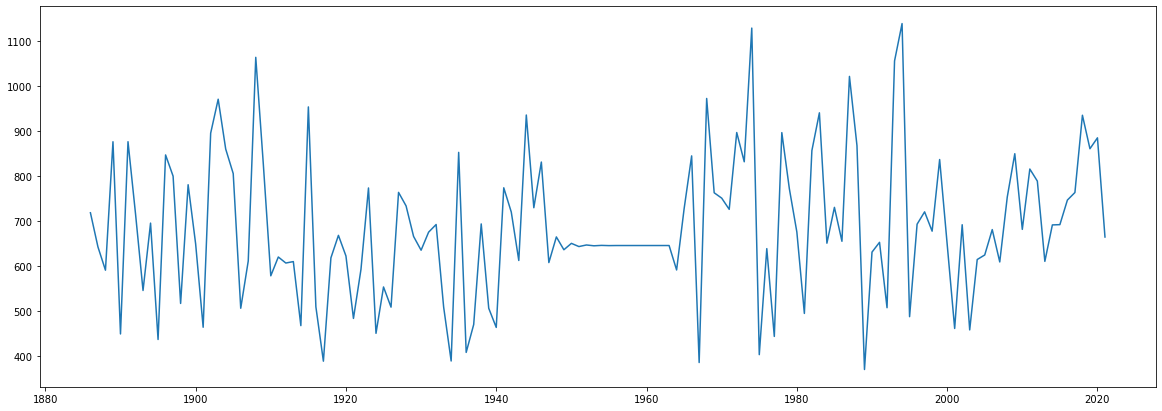
\includegraphics[scale=0.45]{images/line.png}
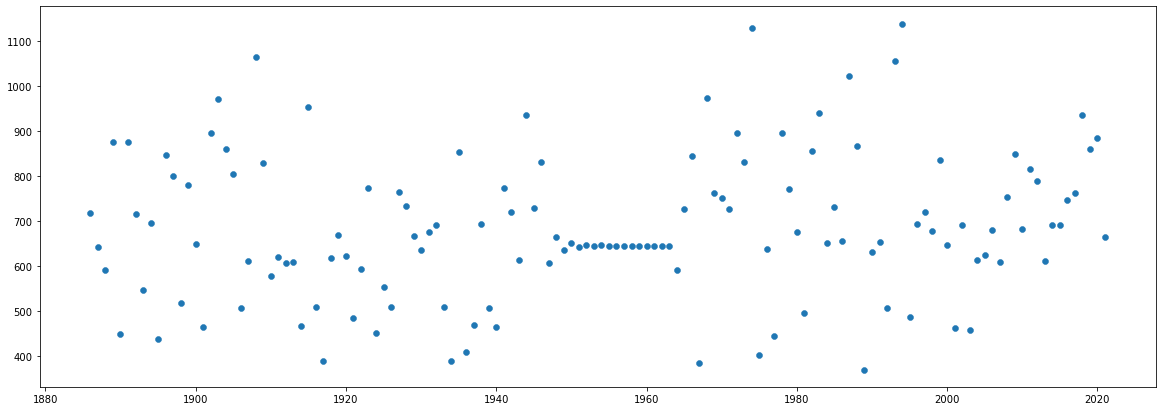
\includegraphics[scale=0.45]{images/scatterplot.png}
\end{center}
\subsection{Mô tả từ dữ liệu}
Ngoại trừ khoảng thời gian số liệu bị khuyết (số liệu của 14 năm, từ năm 1949 đến 1962), đã được tiền xử lý như trình bày trong phần trên, nhìn chung giá trị lượng mưa trung bình năm ở trạm Concordia Muni AP, Kansas, miền Tây Hoa Kỳ có sự biến động liên tục qua từng năm với những khoảng biến động tương ứng tương đối lớn (trên 300 mm) trong trung bình 2 lần trong 20 năm liên tiếp. 

Lượng mưa tại trạm này được tính trung bình trong khoảng 684.3 mm, độ lệch chuẩn lớn, và lượng mưa trung bình mỗi năm ở trạm này trong khoảng thời gian 1886 đến 2021 là lớn hơn 350 mm.
\end{document}